\section{Experiments}

\subsection{Datasets}
The dataset that we will be using is an integrative resource of chest computed tomography images and clinical features of patients with COVID-19 pneumonia (ICTCF) \cite{ref23} which contains the severity score for each CT lung image. ICTCF contains 127 types of clinical features and laboratory confirmed cases of COVID-19 from 1170 patients. The dataset can be found here: http://ictcf.biocuckoo.cn/ . 

The datasets that we will be using to compare with for the segmentation results will be the datasets from Inf-Net\cite{ref14} and the datasets from medseg\cite{ref26}. The dataset from Inf-Net\cite{ref14} contains 68 labeled CT images while the dataset from medseg contains 911 labeled CT images. In total, the number of labeled segmented CT images is 979.

The other datasets that we will be focusing on are COVID-CT-Dataset \cite{ref21} and covid-chestxray-dataset \cite{ref22}. COVID-CT-Dataset can be found at https://github.com/UCSD-AI4H/COVID-CT. COVID-CT-Dataset consist of 349 CT images obtianed from 216 patients. Covid-chestxray-dataset can be found at https://github.com/ieee8023/covid-chestxray-dataset. COVID-CT-Dataset  was created through assembling medical images from publications and websites and contains 123 frontal view X-rays of the lungs. An additional dataset that we can use is from Cell \cite{ref24}, http://ncov-ai.big.ac.cn/download?lang=en if we have enough capacity to load the dataset as the dataset can be huge. This dataset is constructed from the China Consortium of Chest CT Image investigation (CC-CCII). The CT images are classified into novel coronavirus pneumonia (NCP) caused by SARS-CoV-2 virus, common pneumonia and normal controls. It consists of 617,775 CT images obtained from 4,154 patients.

\subsection{Data Augmentation}
We used data augmentation to increase our data samples size. The data agumentation that we used includes \textit{vertical flipping, horizontal flipping, random crop, and random cutout}. For the random cutout percentage, we experimented that 0.5 cutout of the CT lung images yield higher performance than the rest of the value. This is because entropy at 0.5 is the highest which could increase more variability of the images. Examples of the data augmentation can be seen in figure \ref{fig:data_aug}.

\begin{figure}
	\centering
	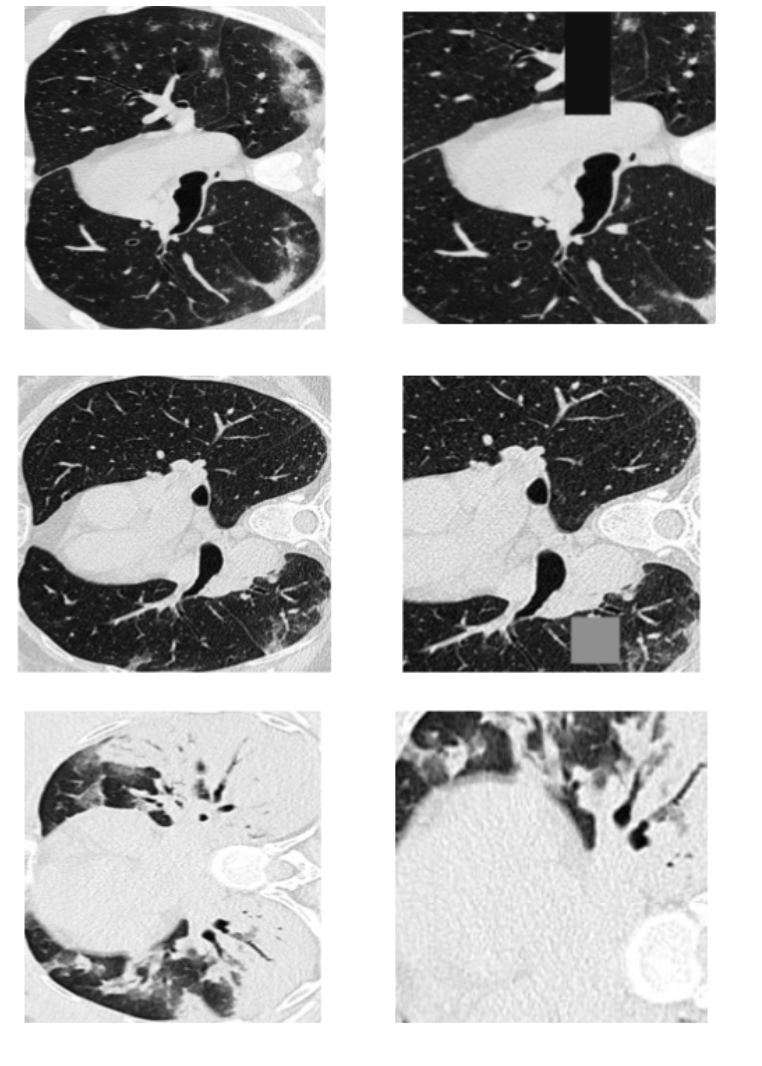
\includegraphics[width=\linewidth]{data_aug.png}
	\caption{Example CT lung images of our data augmentation. The left column is the original CT lung images while the right column is the augmented CT lung images. The first row of the CT lung images involves random cropping and random cutout. The second row of the CT lung images involves random cropping and random cutout. The third row of the CT lung images involves random cropping and vertical flipping. We can see the random cutout involves patching the image with colors of the same value of rgb. For instance, if the value of r is 10, then the value of g and b are also 10. If the value of r is 50, then the value of g and b are also 50.}
	\label{fig:data_aug}
\end{figure}

\subsection{Performance evaluation of image segmentation}
We have trained the supervised inf-net as baseline with comparison to the supervised inf-net with additional data augmentation. The comparison for the methods can be seen in \ref{tab:table_compare}. We can see that the additional data augmentation improves the performance of the baseline model. For the single segmentation Inf-Net comparison, we can see the performance of the single segmentation Inf-Net improves the most when the random cutout is set to a value of 0.5 without any self-supervised training. 

However, the loss calculation does not truly evaluate the performance of the model. We use an additional performance metrics to calculate the model performance. The performance metrics we will be using is called dice similarity coefficient. As shown in \ref{tab:dice_compare}, we see that the best performing model is the self-supervised single Inf-Net using the dice similarity coefficient. 

\subsection{severity estimation results}


\begin{table}
	\centering

	\begin{tabular}{|l|l|l|}
		\hline
		& single Inf-Net & multi Inf-Net \\\hline
		SInfNet & \textbf{0.60} & 0.93  \\\hline
		SInfNet+data aug (0.4)& 0.67 & 2.74  \\\hline
		SInfNet+data aug (0.5)& 0.65 & 1.66 \textbf{} \\\hline
		Self-super & 0.67 & \\\hline
		Self-super+data aug & 0.71 & \\
		\hline
		
	\end{tabular}
	\caption{Comparison of supervised inf-net (SInf-Net) model with added data augmentation. The values listed in the table represent the test loss. The floating value  after the data augmentation refers to the fraction of the image randomly cutout. 0.2 shows that 0.2 of the image is cutout to be empty. }
	\label{tab:table_compare}
\end{table}

\begin{table}
	\centering
	
	\begin{tabular}{|l|l|l|}
		\hline
		& single Inf-Net & multi Inf-Net \\\hline
		SInfNet &  0.26 & 0.12  \\\hline
		SInfNet+data aug (0.4)&  0.31 & 0.66  \\\hline
		SInfNet+data aug (0.5)& 0.30 & 0.62 \textbf{} \\\hline
		Self-super & 0.31  & \\\hline
		Self-super+data aug & \textbf{0.34} & \\
		\hline
		
	\end{tabular}
	\caption{Comparison of supervised inf-net (SInf-Net) model with added data augmentation. The values listed in the table represent the  dice similarity coefficient. The floating value  after the data augmentation refers to the fraction of the image randomly cutout. 0.2 shows that 0.2 of the image is cutout to be empty. }
	\label{tab:dice_compare}
\end{table}

\iffalse
\begin{table*}[t]
	\centering
	\small
	\begin{tabular}{|l|l|}
		\hline
		Sub-Tasks & Time  \\\hline
		Research on related self-supervised tasks to incorporate the methods into COVID-19 pixel-level image segmentation & 1 week  \\\hline
		Find related COVID-19 dataset for classification labels(for self-supervised) and pixel-level segmentation(for classification) labels & 1 week  \\\hline
		Find baseline methods to compare against & 2 week  \\\hline
		Implement self-supervised method for pixel-level segmentation on COVID-19 segmentation & 3 week  \\\hline
		Experiment and training (including calculating the severity score for lung regions) & 3 week  \\\hline
		Write and finalize paper if successful & 2 week  \\\hline
		
	\end{tabular}
	\caption{Tasks scheduled}
	\label{tab:2}
\end{table*}
\fi